%%==================================================
%% chapter04.tex for SJTU Master Thesis
%% based on CASthesis
%% modified by wei.jianwen@gmail.com
%% version: 0.3a
%% Encoding: UTF-8
%% last update: Dec 5th, 2010
%%==================================================

% \bibliographystyle{sjtu2} %[此处用于每章都生产参考文献]
\raggedbottom
\chapter{DiffCon的设计与实现}
\label{chap:designandimpl}

\section{引言}

前文总结了课题相关的基础算法和优化思路之间的联系和启发,探讨了范围查询需求和算法的数据组织形式之间的关联点,本章节以优化频率矩阵加噪模型、提升发布数据可用性为目的,论述解决方案——非交互式差分隐私匿名优化算法DiffCon的设计和实现。

本章结构安排:首先由基础算法DiffGen的相关特性入手,推导证明DiffGen具有一维直方图特性的理论基础;然后介绍具体的设计实现细节,从设计新的应答查询模式、重定义全局敏感性以及基于一致性约束的噪音调整算法这三个方面介绍DiffCon算法,并就其关键技术、难点等作分析;最后进行算法总结、性能的理论分析。

\section{理论基础}

DiffGen算法是本课题的基础算法,优化设计的参照体。基于前文对DiffGen算法的论述,本小节先总结了其数据发布模型所具有的相关性质,然后推出DiffGen模型具有一维直方图特性的结论,并给出严禁证明。一维直方图特性是优化算法DiffCon的理论基础,确保了算法的正确性。

\subsection{DiffGen框架的相关特性}

每个叶节点上的数据项在DiffGen分类树上是唯一出现的,可通过简单的反证法证明。
\subsubsection{唯一性}
\begin{prop}
	\label{chap4_prop1}
	(DiffGen框架的唯一性)DiffGen分类树中,叶节点的属性值分布具有唯一性,即在所有叶节点上,不存在相同的两个数据项。
\end{prop}
\begin{proof}
	假设命题\ref{chap4_prop1}为假,即在DiffGen分类树中,存在两个相同属性值分布的叶节点,也就是对于某一属性值集合为\{a,b,c\}的叶节点A,存在另一属性值集合为\{a,b,c\}的叶节点B,且A,B不为同一节点。
	
	根据分类树,寻找A,B的最小公共祖先节点C,得到节点C的分裂属性Ca及Ca的匿名树。由于A与B相交,显然Ca的匿名树在Ca上的划分产生了两个一样的属性值x,x$\in$\{a,b,c\}。具有重复属性值x的结论与匿名树的定义矛盾。因此,命题\ref{chap4_prop1}为真。
\end{proof}
此特性决定了针对某一属性范围的节点组合是非冗余的,保证了组合结果的唯一合法性。否则,查询结果会存在二义性问题,使得查询请求返回失败。

\subsubsection{完整性}

\begin{prop}
	\label{chap4_prop2}
	(DiffGen框架的完整性)DiffGen分类树的构建过程中,每次属性的划分具有完整性,即对于某次分裂$v$$\rightarrow$$child(v)$,$child(v)$中的每个属性值在$Cut_{i}$中能够完整更新。
\end{prop}
\begin{proof}
	在DiffGen算法\ref{diffgen}的第7行,对挑选节点$v$的分裂操作是严格按照匿名树定义进行的。因此对于$\forall$ $cv$ $\in$ $child(v)$,必然有$cv$ $\in$ $Cut_{i}$。
\end{proof}

\subsubsection{健壮性}

属性划分的完整性确保了在各种合法查询请求中,DiffGen框架的绝对健壮性,首先定义合法查询如下。

\begin{defn}
	(合法查询)有d个属性的数据集,属性$A_{i}$的匿名树上的所有属性值集合为$T_{i}$,$i$ $\in$ [1,d],则所有匿名树的属性值集合$T_{total}$ = $\sum\limits_i^d \cup T_{i}$。
	基于属性值区间的查询能够拆分成若干个属性值的组合,因此某查询请求$Q$可表示成涉及$k$个不同的属性值查询,$Q$=$\{a_{1},a_{2},...,a_{k}\}$,其中k $\leqslant$ |$T_{total}$|,$a_{k}$为属性值。若查询$Q$满足以下条件,则$Q$为合法查询:
	\begin{equation}
	\text{对于}\forall a_{i} \in Q, i \in [1,k], \text{总有}a_{i} \in T_{total}
	\end{equation}
\end{defn}

\begin{prop}
	\label{chap4_prop3}
	(DiffGen框架的健壮性)对于任意的合法查询,DiffGen返回的应答结果具有绝对健壮性,即对于查询序列中的任一属性值查询,均能在DiffGen分类树上找到应答节点。
\end{prop}
\begin{proof}
	设属性$A$的某一属性值$a$为某个合法查询请求中的查询属性值,且$A$的匿名树结构中$a$的父节点集合为$Fa$,$Fa$为根节点到$a$路径上的属性值集合。若$a$为根节点,即$a$=$Fa$,显然$a$就出现在分类树根节点上,应答节点即为根节点。若$a$$\neq$$Fa$,则$a$在分类树上有两种表现形式。(1)$a$在匿名树上的直接父节点属性值发生了分裂,由于\label{chap4_prop2}属性划分的完整性,则必然能在分类树上找到属性值为$a$的节点。(2)若$a$的间接父节点发生分裂或者属性$A$从未被选中,则在分类树上没有属性值为$a$的节点。但由于$a$$\in$$Fa$,那么在分类树中总能找到应答节点,它在$A$上的属性值为$Fa$中离$a$最近的父节点属性值,最坏情况下返回根节点作为应答。
	因此,对于合法查询请求中的任一属性值,在DiffGen分类树上总存在可覆盖此属性值的节点,保障所有查询项的完整性。
\end{proof}

DiffGen框架的健壮性,保障了对于任意的待查询项,在DiffGen分类树中总能找到完整覆盖其属性值的应答节点,达到对于合法查询有求必应的效果,是证明DiffGen框架具有一维直方图特性的关键性质。

\subsubsection{一致性}

\begin{prop}
	\label{chap4_prop4}
	(DiffGen框架的一致性)在DiffGen分类树上,节点上的数据项之间具有一致性特性,可通过节点的组合运算应答合法查询请求。
\end{prop}
\begin{proof}
	叶节点上属性分布的唯一性保证了应答结果是非冗余的,匿名树和决策树算法的构建过程保证了严格的层级和泛化包含关系,结合\label{chap4_prop2}、\label{chap4_prop3}得证。
\end{proof}

基于分类树结构,健壮性和一致性特性使得对于任一查询项总能找到应答节点或节点集,保证了组合树节点作为应答返回方案的可行性。可替换原有的叶节点叠加应答模式,利用$BoostH$的一致性约束方案提升发布数据的准确度,利用节点属性间的泛化关系设计新的应答模式。

%基于差分隐私的组合性质,在论文\cite{DiffGen}中证明了DiffGen满足$\varepsilon$-差分隐私,并且叶节点数据项之间是相互独立的。

\subsection{一维直方图特性} %正确性讨论,花了这么大力气一堆命题,就是为了说明可利用boost的思路

%最好能搞成命题啊1,范围覆盖,2相互独立(基于差分隐私组合性质)

一维直方图发布模型的特点在于能够响应所有的合法查询请求,对于属性值的范围查询能够通过一系列柱状条的叠加得到,并且单个柱状条计数值的增减改变是不影响其他柱状条的。而在多属性直方图中,随着属性值的增加使得数据集的数据域尺寸变大,柱状条的叠加难以满足所有的合法查询请求,健壮性得不到保障;并且,由于多属性的影响,在属性值的范围查询中每个柱状条之间相互影响,全局敏感性不为1。

\begin{prop}
	\label{chap4_prop4}
	(DiffGen框架的一维直方图特性)DiffGen模型具有一维直方图特性,即在范围查询需求中,DiffGen模型的应答健壮性和发布数据项之间的独立性满足一维直方图特征。
\end{prop}
\begin{proof}
	首先,在应答返回结果上,DiffGen框架具有绝对健壮性和一致性。可通过有限次数的单位数据项组合给合法查询做出应答,使得DiffGen发布的数据项在X轴属性组合上满足一维属性特性。因此,虽然节点中的数据项包含多个属性,但不存在多属性直方图健壮性缺失的问题。%它确保了可通过组合发布的叶节点数据项来应答所有的合法查询请求,
	其次,DiffGen分类树的构造过程满足差分隐私的水平组合特性\ref{parallel}。由于DiffGen分类树从根节点到叶节点路径构成的数据集两两之间不相交,因此需按树高对隐私预算进行切分,这决定了在应答查询请求时,各叶节点内的数据属性分布在组合处理时是相互独立的(论文\cite{DiffGen}已证明),不因多属性分布的影响产生关联,每个叶节点代表单位长度数据项。
	最后,从多维的类属性分布的Y轴上看,DiffGen模型是多个一维类属性直方图的组合,多个类属性不影响一维直方图特性。如例\ref{chap3_exmp}中,可拆分成“已被录用”和“未被录用”两个类属性的一维直方图。
\end{proof}

基于本节的唯一性、完整性、健壮性、一致性和差分隐私组合特性的讨论,最终引出DiffGen模型本质上具有一维直方图特性的结论,说明了借鉴$BoostH$的基于一致性约束的优化思路是可行的。
对于范围计数查询需求,与$BoostH$相同的一维直方图模型特性和一致性约束的理论基础,确保了DiffCon优化算法的正确性。


\section{基于一致性约束的优化算法DiffCon}

%从设计新的应答查询模式、重定义全局敏感性以及基于一致性约束的噪音调整算法

针对范围计数查询应用,基于上节的理论证明,本节就一致性约束的优化思路,对非交互式差分隐私优化算法DiffCon的整体设计进行详细阐述。主要分为以下几个部分:
\begin{enumerate}
	\item 立足于DiffGen的分类树结构,构建辅助树结构$DTree$。它是对原数据集进行重匿名、划分,对噪音分布进行优化调整以及定义新的应答查询模式的基础。
	\item 基于树结构的最小顶点覆盖集算法$TMSC$,设计新的应答查询模式,并重定义全局敏感性。
	\item 实现基于任意树结构的噪音调整算法$DiffConOpt$,作为初步加噪操作后的后置处理算法。
	%\item 在基于单位数据项的数据集发布方式对合法查询请求进行应答的场景中,深入分析DiffCon所采用的组合应答模式的原理——利用分类树结构与一致性特性返回较优结果。
\end{enumerate}


\subsection{辅助树结构}

DiffGen分类树包含了各属性属性值间的匿名泛化关系及节点间的一致性联系,噪音分布、优化技术以及应答查询原理均基于此。因此,以DiffGen的匿名树设计和分类树构建算法为基础,DiffCon维护辅助树结构$DTree$。它可以看成是加噪、发布处理前完整的DiffGen分类树,但是额外维护了$LapNoise$和$OptNoise$两个变量,分别表示初始时的拉普拉斯噪音量和调整优化后的噪音量。定义$DTree$结构的C++风格代码如下,展示了其中的主要变量:

\begin{lstlisting}[language={C++}, caption={DTree结构伪代码}]
struct DTree{
	double $LapNoise$;
	double $OptNoise$;
	set<AttributePartition> $Cut_{i}$;
	vector<DTree*> children;
}
\end{lstlisting}
其中,"AttributePartition"为属性类型,$Cut_{i}$的意义与DiffGen算法\ref{diffgen}中的相同,是所有匿名树中可分裂的属性集合。在分类树构建过程中,通过维护$Cut_{i}$的同步更新,确保$DTree$中的节点与DiffGen分类树节点一一对应,保障分类过程的正确性和完整性。

DiffCon算法的整体流程基于$DTree$树结构,通过决策树算法在$DTree$上对数据集进行匿名化划分,在叶节点添加拉普拉斯噪音。除了维护$LapNoise$和$OptNoise$两个变量,这个过程和DiffGen算法基本一样。然后运行噪音分布优化算法$DiffConOpt$。最后在叶节点上返回真实计数值和$OptNoise$的运算和。DiffCon算法的整体流程\ref{diffcon1}概括如下:

\begin{algorithm}
	\caption{DiffCon算法整体流程} 
	\label{diffcon1}
	\begin{algorithmic}[1]
		\REQUIRE 隐私代价$\varepsilon$,树高$TH$,数据集$D$。
		\ENSURE 新的匿名数据集$\hat{D}$。
		\STATE 初始化分类树根节点、$Cut_{i}$集合,均分$\varepsilon$
		\STATE 初始化$DTree$的根节点$DTree_{R}$,并且$DTree_{R}->Cut_{i}$ $\leftarrow$ $Cut_{i}$
		\FOR{i = 1 to $TH$,$DTree_{i}$表示$DTree$树的第i层节点集}
		\STATE 按DiffGen算法处理连续属性的分裂点,计算$Cut_{i}$中属性的分值并选出属性$v$,同时维护$Cut_{i}$
		\FOR{对于$DTree_{i}$中的每个节点$DTree_{node}$}
		\IF{$v$ $\in$ $DTree_{node}$->$Cut_{i}$} 
		\FOR{每个$cv$ $\in$ $child(v)$}
		\STATE 构建节点$Node_{cv}$,$Node_{cv}$->$Cut_{i}$ $\leftarrow$ $DTree_{node}$->$Cut_{i}$ $ - $ $v$ $\cup$ $cv$
		\STATE $DTree_{node}$->$children$ $\leftarrow$ $DTree_{node}$->$children$ $\cup$ $Node_{cv}$
		\ENDFOR
		\ENDIF 
		\ENDFOR
		\ENDFOR
		\STATE 往$DTree$的每个叶节点上加$LapNoise$噪音,$LapNoise$ = Laplace($S(DiffCon)$/$\varepsilon$)
		\STATE 在$DTree$上运行优化算法$DiffConOpt$
		\RETURN 在叶子节点的数据项上,类属性真实计数值为$C$,返回($C$+$OptNoise$))
	\end{algorithmic}
\end{algorithm} 

在算法\ref{diffcon1}中,属性的处理和选择均基于DiffGen算法,保证分类树和$DTree$树的同步构建。从第5行开始,对于挑选出的属性$v$,按照分裂$v$$\rightarrow$$child(v)$,为当前节点的构造子节点集。以此属性的匿名树为依据,有|$child(v)$|个属性则有|$child(v)$|个子节点,在第7行针对每个属性构建子节点,第8行更新节点的$Cut_{i}$域。第14行更新$LapNoise$变量,其中$S(DiffCon)$为重定义的全局敏感性,将在下一小节详细说明。在第15行运行优化算法$DiffConOpt$之后,$OptNoise$为优化后的噪音量,它将替代$LapNoise$在第16行与类计数的真实值做相加运算,最后返回并生成发布数据集。

\subsection{重定义查询应答模式}

继\ref{LP_publish}节对直方图发布方式的论述,本节首先对合法查询请求做量化定义,然后基于范围查询需求和相同的数据发布格式,从误差方差角度比对直方图与基于$TMSC$算法的应答查询模式的区别,并证明重定义的全局敏感性,确保不失差分隐私定义。

\subsubsection{合法查询请求}

合法查询请求$\mathcal{Q}$有m个查询项,$[x,y]$表示对于属性值区间$[x-y]$的范围计数查询,$[x,x]$表示单位长度查询。例如,在直方图\ref{fig:histogram}中,[15,15]和[19,19]均表示对于[15-19]数据项的查询,[15,24]表示对[15-24]的年龄范围查询。
因此查询$\mathcal{Q}$表示为
\[
\mathcal{Q} = \{C([x_{1},y_{1}]),C([x_{2},y_{2}]),...,C([x_{m},y_{m}])\}
\]
其中,$\|x_{i}\|_{1} = 1, \|y_{i}\|_{1} = 1, x_{i} \leqslant y_{i}$

\subsubsection{一维直方图的查询应答方式}

一维直方图的计数统计可用一系列单位长度项的集合$\mathcal{H}$表示。数据集$D$中共有n个行项(柱状条),每个行项$e_{i}$(i$\in$[1,n])的计数值为$C(e_{i})$,那么序列$\mathcal{H}$可表示为
\begin{equation*}
	\mathcal{H} = \{C(e_{1}),C(e_{2}),...,C(e_{n})\}
\end{equation*}
其中,$\|x_{i}\|_{1} = 1$。

\begin{exmp}
	\label{chap4_exmp}
	直方图\ref{fig:histogram}可表示为$\mathcal{H}$ = $\{C([15-19]),C([20-24]),C([25-29],C([30-34]),C([35-40])\}$,更进一步$\mathcal{H}$ = \{1,2,3,0,2\}。
\end{exmp}

由全局敏感性的定义,改变某一项$C(x_{i})$得到数据集$D'$,$D$与$D'$在计数查询上的L1距离为1,因此全局敏感性$S(\mathcal{H})$=1。那么以下的基于拉普拉斯加噪算法满足$\varepsilon$-差分隐私:
\begin{equation}
	\label{chap4_lap}
	\tilde{\mathcal{H}}(D) = \mathcal{H}(D) + \textit{Laplace}(1/\varepsilon)^n
\end{equation}

根据\ref{chap2_Linaer}的论述,$\tilde{\mathcal{H}}(D)$的发布格式处理查询需求$\mathcal{Q}$时,属于线性累加的应答查询模式($LinearR$)。因此,对$\mathcal{Q}$中的单个查询项$C([x_{i},y_{i}])$进行应答处理时,返回的应答结果$A_{i}(D)$为
\begin{equation}
\label{chap4_answer}
\begin{split}
	A_{i}(D) &= \sum\limits_j \widetilde{C}(e_{j})\\
			 &= \sum\limits_j C(e_{j}) + \sum\limits_j \textit{Laplace}(1/\varepsilon)
\end{split}	
\end{equation}
其中$ \forall e_{j} \in [x_{i},y_{i}]$ 且 $\bigcup\limits_j e_{j}$ = $[x_{i},y_{i}]$。


由\ref{chap4_answer}式可以看出,用单位长度的计数项应答范围查询时,只能采用线性叠加的方式。因此在返回整个查询序列$\mathcal{Q}$的应答结果中,总的噪音累加量为$\sum\limits_m {\sum\limits_j \textit{Laplace}(1/\varepsilon)}$,是个随着真实值等额叠加的结果。
%应该改为 误差方差的分析,不然TMSC分析不下去了

同样,在误差方差$error_{var}$方面,$\mathcal{Q}$中第i个范围查询项$C([x_{i},y_{i}])$的误差方差$error_{var}^{i}$与$\mathcal{Q}$的总误差方差$error_{var}^{\mathcal{Q}}$为
\begin{equation}
\label{linear_error}
\begin{split}
	error_{var}^{i} &= |y_{i}-x_{i}| \cdotp \mathbb{E}(\textit{Laplace}(1/ \varepsilon)^2) = \frac{2|y_{i}-x_{i}|}{\varepsilon^2} \\
	error_{var}^{\mathcal{Q}} &= \sum\limits_i error_{var}^{i} = \frac{2}{\varepsilon^2}\sum\limits_i |y_{i}-x_{i}|
\end{split}
\end{equation}
可见,误差方差是随着$\mathcal{Q}$的查询维度线性递增的,发布数据的准确性将不断衰减。

\ref{chap4_answer}式与\ref{linear_error}式形象地表述了基于单位长度的发布格式$\mathcal{H}$在噪音总量和误差方差两方面与查询维度的联系,从数学公式上清楚地呈现了发布数据的准确性将与查询维度成反比的糟糕关系。
在接下来的章节中,本课题通过设计新的查询应答模式,在保持原有的单位长度数据项发布格式$\mathcal{H}$的基础上,重定义全局敏感性,优化误差方差。


\subsubsection{基于TMSC算法的查询应答模式}

由上一节的分析可以看到,单位长度数据项的线性组合和噪音的等额叠加是问题的关键所在。若能从这两方面入手,改变线性组合方式并且尽可能地减少噪音叠加的发生,使得噪音运算远少于真实值的运算,那么问题显然可以得到改善。

本课题设计一种基于$DTree$搜索的查询应答模式$TMSC$,利用树节点间的一致性特性,对于满足查询范围的叶节点(单位长度数据项)集合,查找它们的最小公共祖先节点集合作为应答返回。继续使用\ref{chap3_exmp}的例子,其加噪处理前的一致性树状结构如图\ref{fig4:consistency}。为了简化叙述,仅使用针对“年龄”属性的查询作为示例,例\ref{chap4_exam}对基于一致性树状结构的查询应答方式做了具体表述。

\begin{figure}[!htp]
	\centering
	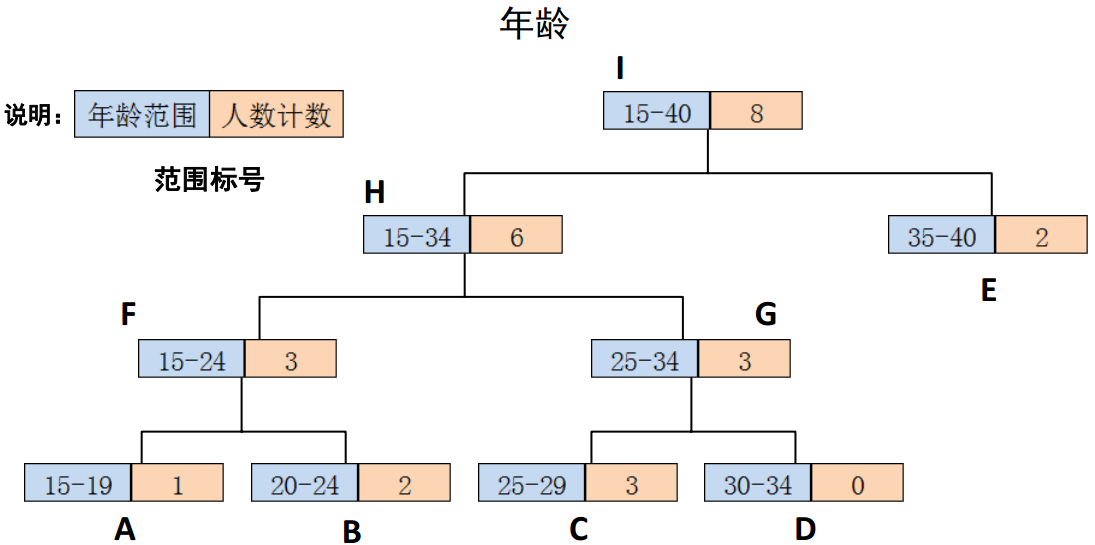
\includegraphics[width=5in]{chap4/examage}
	\bicaption[fig4:consistency]{图}{属性“年龄”的一致性树状结构}{Fig.}{The consistent tree structure for attribute 'Age'}
\end{figure}

\begin{exmp}
	\label{chap4_exam}
数据集发布序列为叶节点数据项集合,即$\tilde{\mathcal{H}}$ = \{$\tilde{C}(x_{A})$,$\tilde{C}(x_{B})$,$\tilde{C}(x_{C})$,$\tilde{C}(x_{D})$,$\tilde{C}(x_{E})$\}。现有查询序列$\mathcal{Q}$=\{C([15-19]),C([20-29]),C([15-34]),C([15-40])\}。那么,对于单位长度查询C([15-19]),直接返回节点A的计数值$\tilde{C}(x_{A})$即可。对于范围查询C([20-29]),由于节点B,C的最小公共祖先节点集为{B,C},因此返回($\tilde{C}(x_{B})$+$\tilde{C}(x_{C})$);对于C([15-34]),其覆盖节点A,B,C,D的最小公共祖先节点集为{H},因此返回$\tilde{C}(x_{H})$;对于C([15-40],同理寻得A,B,C,D,E的最小公共祖先节点集为{I},返回$\tilde{C}(x_{I})$。
\end{exmp}

这其实是一个树结构上的“最小集合覆盖”问题——寻找最小的能够完全覆盖给定的叶节点集合的父节点集。基于贪心思想,$DTree$树结构的最小集合覆盖算法$TMSC$描述如下:

\begin{algorithm}[H]
	\caption{基于$DTree$树结构的最小集合覆盖算法TMSC}\label{euclid}
	\label{msc}
	\begin{algorithmic}[1]
		\REQUIRE $DTree$树结构, 待查询的属性范围$\mathbb{A}$
		\ENSURE 最小覆盖集合$\Upsilon$
		初始化 $\Upsilon$, $\Upsilon$ $\leftarrow$ $\varnothing$
		\FOR{后续遍历$DTree$中的每个叶节点$leaf$}
		\STATE $leaf$的覆盖范围表示为$cover(leaf)$
		\WHILE{$cover(leaf)$ $\subseteq$ $\mathbb{A}$}
		\STATE $leaf_{copy}$ $\leftarrow$ $leaf$
		\STATE $leaf$ $\leftarrow$ $leaf$的父节点
		\ENDWHILE 
		\STATE $\Upsilon$ $\leftarrow$ $\Upsilon$ $\bigcup$ $leaf_{copy}$
		\STATE $\mathbb{A}$ $\leftarrow$ $\mathbb{A}$ $-$ $cover(leaf_{copy})$
		\IF{$\mathbb{A}$ = $\varnothing$}
		\RETURN $\Upsilon$
		\ENDIF
		\ENDFOR
	\end{algorithmic}
\end{algorithm}

算法\ref{msc}中,属性范围$\mathbb{A}$为待覆盖集合,返回集合$\Upsilon$为最小的覆盖集合。算法第2行,后序遍历中仅对叶节点做处理。算法第3-6行,对于覆盖范围包含于集合$\mathbb{A}$的每个叶节点,贪心地向上取尽可能靠近根节点的父节点。第8,9行做更新处理。第10行,当$\mathbb{A}$为空,则表示$\Upsilon$中的节点集已经完全覆盖初始的$\mathbb{A}$,返回即可。

基于$TMSC$查询应答模式的数据发布格式初步方案,在\ref{LP_publish}节中已探讨过,即\ref{L_allnodes}式中发布全部节点信息的$\tilde{L}_{all}$。此处对$\tilde{L}_{all}$的弊端做简要的总结:(1)加噪后的$DTree$丧失一致性特性。(2)泄露了非叶结点的信息,隐私保障力度降低。
因此,后文介绍的$DiffConOpt$算法将对噪音分布进行调整,使得含噪的$DTree$重获一致性特性。因此,采用简单的直方图发布格式$\mathcal{H}$,通过单位长度数据项(叶节点)的叠加运算也能无差别地获取任意非单位长度的数据项(非叶子节点),而不需暴露非叶结点信息。
%从而满足$TMSC$算法中返回父节点计数值的需求。

\subsubsection{重定义全局敏感性}

查询应答方式的改变引起了全局敏感性的改变,因此需要重新定义。

\begin{prop}
	\label{DTreeSensitivity}
	基于$DTree$的查询应答方式的全局敏感性为其树高$DHeight$。
\end{prop}
\begin{proof}
	若增加或移除一个叶节点(单位长度数据项)$leaf$,那么会影响相关查询范围的计数统计情况。这个范围包括:(1)对于命中$leaf$的单位长度查询的范围,范围大小为1;(2)从$DTree$的根节点到叶节点$leaf$路径上的每个节点所覆盖的查询范围,范围大小为树高$TH$。因此,增加或移除一个叶节点$leaf$会影响$TH$个范围计数查询情况,根据全局敏感性定义,$S(DTree)$=$TH$。
\end{proof}

由于敏感性的改变,根据命题\ref{DTreeSensitivity}与式子\ref{L_allnodes},初步发布格式$\tilde{L}_{all}$基于拉普拉斯机制的差分隐私算法具体化为:
\begin{equation}
\label{chap4_dtree}
\tilde{L}_{all}(D) = L_{all}(D) + \textit{Laplace}(TH/\varepsilon)^{ntree}
%\widetilde{\mathcal{H}}(D) = \mathcal{H}(D) + \textit{Laplace}(TH/\varepsilon)^n
\end{equation}
其中,$ntree$为发布序列$\tilde{L}_{all}$的维度,即$DTree$的节点总数。

一般地有$TH$>1,可见此时由于全局敏感性的增加,在叶节点上添加了更大量级的拉普拉斯噪音。因此,基于$TMSC$算法的应答查询模式在给非单位长度的范围查询带来效益的同时,可能会降低单位长度查询结果的准确性。下节介绍的算法$DiffConOpt$能够有效地解决这个问题,它高效地调整噪音分布,哪怕在单位长度查询准确度上的表现依旧优于直方图发布方式。

%从误差方差或者表达式方面与原来的式子进行比对 否则太粗糙了


%引出树的敏感性,小波和boost里边有,给出定义;研究下DiffGen的敏感性

%给图说明新的应答模式

%应说清 为了利用一致性进行应答,因此全局敏感要改,但是还是落在叶节点上。

\subsection{噪音调整算法}

$DTree$节点间的一致性特性是由匿名树泛化关系所决定的节点之间的固有属性,噪音的扰动仅仅是打破了数值等式关系,因此在确保总噪音量不缺失情况下,一致性特性是作为噪音数值调整的依据。
噪音调整算法$DiffConOpt$在DiffCon算法流程中具有三方面作用:(1)经过噪音分布调整后的$DTree$在节点计数值上重获一致性等式关系,这是采用直方图数据发布格式支持$TMSC$查询应答模式的前提。(2)无论对于单位长度的查询还是范围查询,均能提升查询结果的准确度。(3)不失隐私保障力度,保护了$DTree$内部节点的信息安全与联系。

假设$DTree$中的节点$x$的加噪计数表示为$\tilde{x}$,即"LapNoise"变量;调整后的优化结果为$\ddot{x}$,即"OptNoise"变量,中间变量记为$\acute{x}$。以节点$x$为根节点的子树中,其节点总数为$N_{total}(x)$,有$N_{leaf}(x)$个叶节点。$x$的父节点为$P_{x}$,$x$的下一层子节点集合为$ChildSet(x)$。

适用于任意树结构的噪音调整算法$DiffConOpt$是个基于最小二乘法思想的具有一致性特性的优化算法,以下是具体的实现算法\ref{adjustnoise}。

\begin{algorithm}[H]
	\caption{噪音调整算法DiffConOpt} 
	\label{adjustnoise}
	\begin{algorithmic}[1]
		\REQUIRE $DTree$树
		\ENSURE 重获一致性特性且优化噪音分布的$DTree$树
		\FOR{后续遍历$DTree$中的每个节点$x$}
		\IF{ $x$是叶节点}
		\STATE $\acute{x}$ $\leftarrow$ $\tilde{x}$ 
		\ELSE
		\STATE  $\acute{x}$ $\leftarrow$ $\frac{{N_{leaf}(x) * \tilde{x} + (N_{total}(x) - N_{leaf}(x)) * \sum\nolimits_{v \in ChildSet(x)} {\ddot{v}}}}{{N_{total}(x)}}$
		\ENDIF
		\ENDFOR
		\FOR{先序遍历$DTree$中的每个节点$x$}
		\IF{ $x$是根节点}
		\STATE  $\ddot{x}$ $\leftarrow$ $\acute{x}$
		\ELSE
	%	\STATE  $ChildNum$ = ${\sum\nolimits_{v \in Child(x)} {1}}$
		\STATE  $\ddot{x}$ $\leftarrow$ $\acute{x} + \frac{{\ddot{P_{x}} - \sum\nolimits_{v \in ChildSet(P_{x})} {\acute{v}}}}{|ChildSet(P_{x})|}$
		\ENDIF
		\ENDFOR
		\RETURN $DTree$
	\end{algorithmic}
\end{algorithm}

通过两次遍历完成算法DiffConOpt。第一次在算法第1行,自底向上的顺序遍历$DTree$的每个节点,求其优化结果。若非叶节点,则进行第5行的调整处理,否则直接以噪音值作为优化值。第二次采用自顶向下的顺序遍历节点,算法第8行开始,对于非根节点进行第12行的调整处理,否则原值返回;$|ChildSet(P_{x})|$表示集合$ChildSet(P_{x})$的大小,即$P_{x}$的下一层子节点总数。最后,发布重获一致性特性且具有更优噪音分布的$DTree$树。对于调整后的噪音分布,在算法\ref{diffcon1}的第14行,可具体化为$LapNoise$ $\leftarrow$ Laplace($TH$/$\varepsilon$)。

算法\ref{adjustnoise}适用于任意树结构,对$HBoost$的完全$k$-叉树情况做了扩展。

\begin{prop}
	\label{chap4_consistent}
	对于$DTree$上的每个节点$x$,经过式子
	\[
	\ddot{x} = \left\{ 
	{\begin{array}{*{20}l}
		\acute{x},  & {\begin{array}{*{20}l}
			x\text{为叶节点},   \\
			\end{array} }   \\ 
		
		\acute{x} + \frac{{\ddot{P_{x}} - \sum\nolimits_{j \in ChildSet(P_{x})} {\acute{j}}}}{|ChildSet(P_{x})|},  & {\begin{array}{*{20}l}
			x\text{非叶节点}  \\
			\end{array} }  \\  
		\end{array} } \right.
	\]
	后,得每个节点的优化值$\ddot{x}$满足基于一致性约束的最小二乘法目标式
	\begin{equation}
	\label{equa_l2}
	\begin{split}
	minimize \sum\limits_{x \in DTree} (\ddot{x} - \tilde{x})^2 \\
	subject\ \ to\ \ \forall x,\ \ \ddot{x} = \sum\limits_{c \in ChildSet(x)} \ddot{c} 
	\end{split}
	\end{equation}
\end{prop}
\begin{proof}
	对于$DTree$中的除了根节点外的任一节点$x$,其父节点记为$p$,即$p = P_{x}$。以$p$为根的子树$Subtree_{p}$的叶节点集为$LeafSet(p)$。由于一致性特性有
	\begin{equation}
		\label{proof1}
		\begin{split}
		\ddot{p} &= \sum\nolimits_{v \in ChildSet(p)} {\ddot{v}}\\
		&= \sum\nolimits_{l \in LeafSet(p)} {\ddot{l}} 
		\end{split}
	\end{equation}
	因此,有$Subtree_{p}$中的节点$a \in Subtree_{p}$,结合\ref{proof1}的关系式,对于子树$Subtree_{P}$,\ref{chap4_consistent}式等价于
	\[
	\begin{split}
	minimize &\sum\limits_{a \in Subtree_{p}} (\ddot{a} - \tilde{a})^2 \\
	subject\ \ to\ \ \forall a\in Subtree_{p},\ \ \ddot{a} = &\sum\limits_{c \in ChildSet(a)} \ddot{c}\ \text{且}\ \ \ddot{p} = \sum\nolimits_{l \in LeafSet(p)} {\ddot{l}} 
	\end{split}		
	\]
	进一步地,对于节点$a$,用$\sum\limits_{l \in LeafSet(a)} \ddot{l}$替换$\sum\limits_{c \in ChildSet(a)} \ddot{c}$,通过参数代换可转换约束条件为无约束的线性规划问题,有
	\begin{equation}
	\label{proof2}
	\begin{split}
	minimize \sum\limits_{a \in Subtree_{p}} ((\sum\limits_{l \in LeafSet(a)} \ddot{l}) - \tilde{a})^2\\
	subject\ \ to\ \ \ddot{p} = \sum\nolimits_{l \in LeafSet(p)} {\ddot{l}} 
	\end{split}		
	\end{equation}
	利用拉格朗日乘数法处理\ref{proof2}式,记$\lambda$为拉格朗日参数,有
	\[
		minimize \sum\limits_{a \in Subtree_{p}} ((\sum\limits_{l \in LeafSet(a)} \ddot{l}) - \tilde{a})^2 - \lambda(\ddot{p} - \sum\nolimits_{l \in LeafSet(p)} {\ddot{l}})
	\]
	使用对$l$求导的方法求目标式极值。对于每个$LeafSet(p)$中的叶节点$l_{i}$,有
	\begin{equation}
	\label{proof3}
	for\ each\  l_{i} \in LeafSet(p):\ \ 2((\sum\limits_{l_{i} \in LeafSet(a)} \ddot{l_{i}}) - \tilde{a}) = -\lambda 
	\end{equation}
	对于$\forall l \in LeafSet(p)$,叠加\ref{proof3}式,并由$\acute{p}$与$\tilde{p}$的递推式得到$\lambda$的表达式
	\[
		\lambda = -\frac{\ddot{p}-\sum\nolimits_{v \in ChildSet(p)} {\acute{v}}}{|LeafSet(p)|}
	\]
	最后,对$\forall l \in LeafSet(x)$,在$Subtree_{x}$范围内的叶节点,叠加上述等式得到
	\[
	\begin{split}
	\ddot{x} &= \acute{x} - \frac{|LeafSet(p)|}{|ChildSet(p)|}\cdotp \lambda \\
		&= \acute{x} + \frac{|LeafSet(p)|}{|ChildSet(p)|}\cdotp (\frac{\ddot{p}-\sum\nolimits_{v \in ChildSet(p)}{\acute{v}}}{|LeafSet(p)|})\\
		&= \acute{x} + \frac{{\ddot{p} - \sum\nolimits_{v \in ChildSet(p)} {\acute{v}}}}{\sum\nolimits_{v \in ChildSet(p)} {1}}\\
		&= \acute{x} + \frac{\ddot{p} - \sum\nolimits_{v \in ChildSet(p)}{\acute{v}}}{|ChildSet(p)|}\\
	\end{split}
	\]
	
	当$x$为根节点时,其父节点$p = \varnothing$。因此\label{proof1}式的$\ddot{p} = 0$,由\ref{proof2}的一致性关系从叶节点出发,同样由拉格朗日乘数法推\ref{proof3}式,易证得
	\[
		\ddot{x} = \acute{x},\ \ x\ is\ DTree's\ root\ node
	\]
	
	综上,命题得证。
\end{proof}

在原始的噪音分布中,由于拉普拉斯加噪是个随机过程,噪音分布不仅不满足一致性关系,并且噪音与真实值之间的距离是“抖动”的——某些节点上的噪音与真实值相差巨大,某些却差距甚小。这种不均衡的噪音分布对噪音误差方差带来了巨大影响。经过算法$DiffConOpt$的调整,噪音分布不仅具有一致性关系,而且分布“平滑”——命题\ref{chap4_consistent}保证了噪音与真实值距离的总平方和最小,整体加噪情况良好。下节通过噪音误差方差的性能分析,将更清楚地看到这点。

\section{性能分析}
\label{theory analysis}
对于查询请求$\mathcal{Q}$中的第i个查询项,我们记\ref{linear_error}式的直方图发布方式的误差方差为$error_{Histog}^{\mathcal{Q}_{i}} = \frac{2|y_{i}-x_{i}|}{\varepsilon^2} = O(\frac{|y_{i}-x_{i}|}{\varepsilon^2})$。对于整个请求$\mathcal{Q}$,其误差方差为$error_{Histog}^{\mathcal{Q}}$
\begin{equation}
\label{linear_error2}
error_{Histog}^{\mathcal{Q}} = O(\frac{\sum\limits_i |y_{i}-x_{i}|}{\varepsilon^2})
\end{equation}

%在初步方案$\tilde{L}_{all}$中,
现在采用基于$TMSC$算法的应答查询模式,对于范围查询$\mathcal{Q}_{i}$,假设$TMSC$算法返回的集合$\Upsilon$=$\{a_{1},a_{2},...,a_{\Upsilon n}\}$。
在初步的数据发布方案$\tilde{L}_{all}$中,由误差方差定义有
\[
	error_{\tilde{L}_{all}}^{a_{j}} = \frac{2 \cdotp TH^2}{\varepsilon^2} = O(\frac{TH^2}{\varepsilon^2})
\]
其中 j = 1,2,..,$\Upsilon n$。

假设$DTree$中节点的最大分支数为$k$,那么$DTree$的节点总数$N_{total}$是与树高$TH$呈倍数关系,$N_{total}$ = $O(k \cdotp TH)$。例如完全三叉树时$N_{nodes}$ = $\Theta(3 \cdotp TH)$。因为经验公式及实际使用中,定义的匿名树的最大分支数通常都在个位数范围内,以防止通过决策树算法生成的分类树产生过度拟合(Overfitting)\cite{overfitting}问题,而且基于决策树算法构建的$DTree$,分支数太多的属性值是很难被挑选到的。因此,在整个请求$\mathcal{Q}$中,集合$\Upsilon$在$\tilde{L}_{all}$上的误差方差$error_{\tilde{L}_{all}}^{\mathcal{Q}}$为

\[
\label{Lall_error}
error_{\tilde{L}_{all}}^{\mathcal{Q}} = \sum\limits_{j \in \Upsilon} error_{var}^{a_{j}}=O(\frac{TH^3}{\varepsilon^2})
\]

%1,说明单位长度也好。2,范围上的好处
现在讨论经过算法$DiffConOpt$优化后的应答查询模式,表示为$\tilde{\mathcal{H}}_{opt}$,其误差方差为$error_{\tilde{\mathcal{H}}_{opt}}^{\mathcal{Q}}$。

\begin{prop}
	\label{chap4_prop5}
	$error_{\tilde{\mathcal{H}}_{opt}}^{\mathcal{Q}} = O(\frac{TH^3}{\varepsilon^2})$
\end{prop}
\begin{proof}
	根据高斯-马尔科夫定理(Gauss–Markov theory)\cite{gauss_markov},最小二乘估量值是具有最小方差的估量。在\ref{equa_l2}式中,$\ddot{x}$是$\tilde{x}$的最小二乘估量值。由$\tilde{x} \in \tilde{L}_{all}(D)$,则$error_{\tilde{\mathcal{H}}_{opt}}^{\ddot{x}} \leqslant error_{\tilde{L}_{all}}^{\tilde{x}} = \frac{2 \cdotp TH^2}{\varepsilon^2}$。对$\mathcal{Q}$中的任一项$C([x_{i},y_{i}])$,最多通过$k\times TH$个节点的组合能返回应答。因此有$error_{\tilde{\mathcal{H}}_{opt}}^{\mathcal{Q}} \leqslant k \times TH \times \frac{2 \cdotp TH^2}{\varepsilon^2} = O(\frac{TH^3}{\varepsilon^2})$。
\end{proof}

进一步,比较$error_{\tilde{\mathcal{H}}_{opt}}^{\mathcal{Q}}$与$error_{\tilde{L}_{all}}^{\mathcal{Q}}$的大小关系。由于$k$仅仅表示最大分支数的取值,其他节点的分支数不确定,并且查询范围的细微区别也能使得应答集合$\Upsilon$大大不同,因此在大小比较与证明上通过$k$值和$TMSC$的最差应答策略取上届(Bound)关系式。

\begin{prop}
	\label{chap4_prop6}
	$error_{\tilde{\mathcal{H}}_{opt}}^{\mathcal{Q}} \leqslant \frac{3 \cdotp error_{\tilde{L}_{all}}^{\mathcal{Q}}}{2(k-1)(TH-2)+k}$
\end{prop}
\begin{proof}
	假设$DTree$的所有叶节点表示范围为[x,y],$\mathcal{Q}$中的某查询项$\mathcal{Q}_{i}$的查询范围为[x+1,y-1],也就是说$\mathcal{Q}_{i}$的涉及了除最左叶节点$l_{left}$、最右叶节点$l_{right}$以外的所有其他节点。由于不能充分利用一致性特性寻找最大覆盖集,因此这种情况是$TMSC$算法采取最差的应答策略情况。
	
	当$DTree$的两两叶节点间除了根节点外均无的同一父节点,即除了根节点找不到比叶节点表示范围更大的覆盖节点,覆盖率为0。
	对于$\tilde{L}_{all}$来说,只能通过叶节点的累加结果作返回。因此,$error_{\tilde{L}_{all}}^{\mathcal{Q}_{i}} = (y-x-2) \cdotp TH^2/\varepsilon^2$,表现为最差的噪音等额叠加现象。
	对于$\tilde{\mathcal{H}}_{opt}$来说,通过运算$\tilde{\mathcal{H}}_{opt}(\text{根节点}) - \tilde{\mathcal{H}}_{opt}(l_{left}) - \tilde{\mathcal{H}}_{opt}(l_{right})$即可返回答案,因此$error_{\tilde{\mathcal{H}}_{opt}}^{\mathcal{Q}_{i}} = \frac{6TH^2}{\varepsilon^2}$。
	
	当$DTree$为$k$叉完全树,此时在每层$Dtree$的中能尽可能多地找到覆盖下层节点的父节点,覆盖率最高。
	对于$\tilde{\mathcal{H}}_{opt}$来说,误差方差不变。
	对于$\tilde{L}_{all}$来说,第一层根节点没有参与应答,第二层仅仅$k$-2个节点参与应答,除此之外的每层有2($k$-1)个节点参与应答,并且共($TH$-2)层。因此,$error_{\tilde{L}_{all}}^{\mathcal{Q}_{i}} = 2(2(k-1)(TH-2)+k-2+2) \cdotp TH^2/\varepsilon^2$。
	
	综上有
	\[
		error_{\tilde{\mathcal{H}}_{opt}}^{\mathcal{Q}_{i}} \leqslant \frac{3 \cdotp error_{\tilde{L}_{all}}^{\mathcal{Q}}}{2(k-1)(TH-2)+k} \leqslant \frac{6 \cdotp error_{\tilde{L}_{all}}^{\mathcal{Q}}}{y-x-2}
	\]
\end{proof}

由命题\ref{chap4_prop6}可以看到,经过噪音分布调整之后的$\tilde{\mathcal{H}}_{opt}$具有更好的误差方差,无论对于单位长度的查询还是范围查询而言,其查询结果均有更高的准确度,发布数据可用性更强。

\section{算法小结}

本章节对DiffCon算法的具体设计和实现进行了详细阐述,现在就算法运行流程和关键细节做分析总结。

首先,基于DiffGen分类树实现的$DTree$树是算法的结构基础,它呈现了各属性属性值间的匿名泛化关系及节点间的一致性联系,并且维护了“LapNoise”和“OptNoise”变量,为噪音优化算法$DiffConOpt$的运行做铺垫。

接下来,改变直方图发布方式的应答查询模式$LinearR$,通过基于树结构最小集合覆盖算法$TMSC$,设计新的查询应答模式,尽可能减少噪音叠加运算。之后重定义全局敏感性,并且在叶节点上添加拉普拉斯噪音以满足差分隐私。

DiffCon采用简单的一维直方图数据发布格式——基于单位长度数据项($DTree$的叶节点)。但由于加噪处理使得$DTree$节点间在数值上不再满足一致性等式,例如父节点的含噪计数值不等于其所有子节点的累加和。因此,需要对节点的噪音分布进行优化处理。基于两个核心调整公式,$DiffConOpt$算法发散叶节点的噪音到每个树节点上,并作一致性平衡调整。

最后,采用DiffGen算法的发布方式——基于$DTree$的叶节点统计数据项,供范围计数查询类应用使用。

在性能探究方面,关注单位长度查询与范围查询两个角度。无乱是从本章节的理论角度还是下个章节的实验阶段,查询结果的准确度在DiffCon算法中均有所提升,并且在准确度扩展性、发布数据可用性上也有较大幅度的提高。


